%Este trabalho está licenciado sob a Licença Atribuição-CompartilhaIgual 4.0 Internacional Creative Commons. Para visualizar uma cópia desta licença, visite http://creativecommons.org/licenses/by-sa/4.0/deed.pt_BR ou mande uma carta para Creative Commons, PO Box 1866, Mountain View, CA 94042, USA.

\chapter{Problema de valor de contorno}\label{cap_pvc}
\thispagestyle{fancy}

Neste capítulo, discutimos sobre a aplicação do método de diferenças finitas para aproximar a solução de problemas de valores de contorno da forma
\begin{align}
  \alpha(x) u'' &+ \beta(x) u' + \gamma(x) u = f(x),\quad c_1 < x < c_2,\\
  \eta_1 u'(c_1) &+ \theta_1 u(c_1) = g_1\\
  \eta_2 u'(c_2) &+ \theta_2 u(c_2) = g_2
\end{align}
onde a incógnita $u = u(x)$ e os são dados os coeficientes $\alpha(x)\neq 0$, $\beta(x)$, $\gamma(x)$ e a função $f(x)$. Nas condições de contorno, são dados os coeficientes $\eta_1$ e $\theta_1$ não simultaneamente nulos, bem como, os coeficientes $\eta_2$ e $\theta_2$, também, não simultaneamente nulos.

\section{Método de diferenças finitas}\label{cap_pvc_sec_mdf}

Consideramos o seguinte problema linear de valor de contorno
\begin{align}
  \alpha(x) u'' &+ \beta(x) u' + \gamma(x) u = f(x),\quad c_1 < x < c_2, \label{eq:pvc_eq}\\
  \eta_1 u'(c_1) &+ \theta_1 u(c_1) = g_1 \label{eq:pvc_bc1}\\
  \eta_2 u'(c_2) &+ \theta_2 u(c_2) = g_2 \label{eq:pvc_bc2}
\end{align}
onde a incógnita $u = u(x)$ e os são dados os coeficientes $\alpha(x)\neq 0$, $\beta(x)$, $\gamma(x)$ e a função $f(x)$. Nas condições de contorno, são dados os coeficientes $\eta_1$ e $\theta_1$ não simultaneamente nulos, bem como, os coeficientes $\eta_2$ e $\theta_2$, também, não simultaneamente nulos.

A aproximação pelo método de diferenças finitas de \eqref{eq:pvc_eq}-\eqref{eq:pvc_bc2} surge da substituição das derivadas por fórmulas de diferenças finitas. Isto requer a a prévia discretização do domínio do problema. Mais precisamente, a aplicação do método de diferenças finitas envolve três procedimentos básicos: 1. discretização do domínio, 2. discretização das equações, 3. resolução do problema discreto.

\begin{flushleft}
  {\bf 1. Discretização do domínio}
\end{flushleft}

A discretização do domínio refere-se ao particionamento do mesmo em pontos espaçados uniformemente ou não. Aqui, para mantermos a simplicidade, vamos considerar apenas o caso de um particionamento uniforme. Desta forma, escolhemos o número $n$ de pontos da partição e, então, o passo é dado por
\begin{equation}
  h = \frac{c_2-c_1}{n-1},
\end{equation}
e os pontos da partição podem ser indexados da seguinte forma
\begin{equation}
  x_i = c_1 + (i-1)h.
\end{equation}

\begin{flushleft}
  {\bf 2. Discretização das equações}
\end{flushleft}

Começando pela equação \eqref{eq:pvc_eq}, no ponto $x=x_i$ temos
\begin{equation}
  \alpha(x_i) u''(x_i) + \beta(x_i) u'(x_i) + \gamma(x_i) u(x_i) = f(x_i) \label{eq:pvc_eq_no_ponto}
\end{equation}
para $i=2, 3, \dotsc, n-1$. Podemos substituir a segunda derivada de $u$ pela fórmula de diferenças finitas central de ordem $h^2$, i.e.
\begin{equation}
  u''(x_i) = \underbrace{\frac{u(x_i-h) - 2u(x_i) + u(x_i+h)}{h^2}}_{D_{0,h^2}^2u(x_i)} + O(h^2).
\end{equation}
A primeira derivada de $u$ também pode ser substituída pela fórmula de diferenças finitas central de ordem $h^2$, i.e.
\begin{equation}
  u'(x_i) = \underbrace{\frac{u(x_i+h)-u(x_i-h)}{2h}}_{D_{0,h^2}u(x_i)} + O(h^2).
\end{equation}

Agora, denotando $u_i \approx u(x_i)$, temos $u_{i-1}\approx u(x_i-h)$ e $u_{i+1}\approx u(x_i+h)$. Então, substituindo as derivadas pelas fórmulas de diferenças finitas acima na equação \eqref{eq:pvc_eq_no_ponto}, obtemos
\begin{align}
  \alpha(x_i)\left(\frac{u_{i-1}-2u_i+u_{i+1}}{h^2}\right) &+ \beta(x_i)\left(\frac{u_{i+1}-u_{i-1}}{2h}\right) \nonumber \\
  &+ \gamma(x_i)u_i + O(h^2) = f(x_i),
\end{align}
para $i=2, 3, \dotsc, n-1$. Rearranjando os termos e desconsiderando o termo do erro de truncamento, obtemos o seguinte sistema discreto de equações lineares
\begin{align}
  \left(\frac{\alpha(x_i)}{h^2}-\frac{\beta(x_i)}{2h}\right)u_{i-1} &+ \left(\gamma(x_i) - \frac{2\alpha(x_i)}{h^2}\right)u_i \nonumber \\
  &+ \left(\frac{\alpha(x_i)}{h^2}+\frac{\beta(x_i)}{2h}\right)u_{i+1} = f(x_i), \label{eq:pvc_mdf_sis1}
\end{align}
para $i=2, 3, \dotsc, n-1$. Observe que este sistema consiste em $n-2$ equações envolvendo as $n$ incógnitas $u_i$, $i=1, 2, \dotsc, n$. Para fechá-lo, usamos as condições de contorno.

Usando a fórmula de diferenças finitas progressiva de ordem $h^2$ para a derivada $u'(c_1)$ temos
\begin{equation}
  u'(c_1) = \frac{-3u(c_1) + 4u(c_1+h) - u(c_1+2h}{2h} + O(h^2).
\end{equation}
Então, observando que $c_1$ corresponde ao ponto $x_1$ na partição do domínio, temos $u_1 \approx u(c_1)$, $u_2 = u(c_1+h)$ e $u_3 = u(c_1+2h)$ e, portanto de \eqref{eq:pvc_bc1} temos
\begin{equation}
  \eta_1\left(\frac{-3u_1 + 4u_2 - u_3}{2h}\right) + \theta_1u_1 + O(h^2) = g_1.
\end{equation}
Então, desconsiderando o termo do erro de truncamento, obtemos a seguinte equação discreta
\begin{equation}
  \left(\theta_1 - \frac{3\eta_1}{2h}\right)u_1 + \frac{2\eta_1}{h}u_2 - \frac{\eta_1}{2h}u_3 = g_1.\label{eq:pvc_mdf_sis0}
\end{equation}

Procedendo de forma análoga para a condição de contorno \eqref{eq:pvc_bc2}, usamos a fórmula de diferenças finitas regressiva de ordem $h^2$ para a derivada $u'(c_2)$, i.e.
\begin{equation}
  u'(c_2) = \frac{3u(c_2) - 4u(c_2-h)+u(c_2-2h)}{2h} + O(h^2).
\end{equation}
Aqui, temos $u_{n}\approx u(c_2)$, $u_{n-1}\approx u(c_2-h)$ e $u_{n-2}\approx u(c_2-2h)$, e de \eqref{eq:pvc_bc2} obtemos
\begin{equation}
  \eta_2\left(\frac{3u_n - 4u_{n-1} + u_{n-2}}{2h}\right) + \theta_2u_n + O(h^2) = g_2.
\end{equation}
Então, desconsiderando o termo do erro de truncamento, obtemos
\begin{equation}
  \frac{\eta_2}{2h}u_{n-2} - \frac{2\eta_2}{h}u_{n-1} + \left(\theta_2 + \frac{3\eta_2}{2h}\right)u_n = g_2.\label{eq:pvc_mdf_sis2}
\end{equation}

Por fim, as equações \eqref{eq:pvc_mdf_sis0}-\eqref{eq:pvc_mdf_sis2} formam o seguinte problema discretizado pelo método de diferenças finitas
\begin{align}
  &\left(\theta_1 - \frac{3\eta_1}{2h}\right)u_1 + \frac{2\eta_1}{h}u_2 - \frac{\eta_1}{2h}u_3 = g_1.\label{eq:pvc_mdf_bc1}\\
  &~\nonumber\\
  &\left(\frac{\alpha(x_i)}{h^2}-\frac{\beta(x_i)}{2h}\right)u_{i-1} + \left(\gamma(x_i) - \frac{2\alpha(x_i)}{h^2}\right)u_i \nonumber \\
  &+ \left(\frac{\alpha(x_i)}{h^2}+\frac{\beta(x_i)}{2h}\right)u_{i+1} = f(x_i),~i=2, \dotsc, n-1, \label{eq:pvc_mdf_eq}\\
  &~\nonumber\\
  &\frac{\eta_2}{2h}u_{n-2} - \frac{2\eta_2}{h}u_{n-1} + \left(\theta_2 + \frac{3\eta_2}{2h}\right)u_n = g_2.\label{eq:pvc_mdf_bc2}
\end{align}

\begin{flushleft}
  {\bf 3. Resolução do problema discreto}
\end{flushleft}

O problema discreto \eqref{eq:pvc_mdf_bc1}-\eqref{eq:pvc_mdf_bc2} consiste em um sistema linear de $n$ equações com $n$ incógnitas. Na forma matricial temos
\begin{equation}
  A\tilde{u} = b
\end{equation}
onde $\tilde{u} = (u_1, u_2, \dotsc, u_n)$ é o vetor das incógnitas, $b$ é o vetor dos termos contantes $b = (g_1, f(x_2), f(x_3), \dotsc, f(x_{n-1}), g_2)$ e $A$ é a matriz dos coeficientes. Observamos que os coeficientes não nulos da matriz $A$ são:
\begin{align}
  a_{11} &= \left(\theta_1 - \frac{3\eta_1}{2h}\right),\\
  a_{12} &= \frac{2\eta_1}{h},\\
  a_{13} &= - \frac{\eta_1}{2h},\\
  & ~ \nonumber \\
  a_{i,i-1} &= \left(\frac{\alpha(x_i)}{h^2}-\frac{\beta(x_i)}{2h}\right), ~i=2, \dotsc, n-1,\\
  a_{i,i} &= \left(\gamma(x_i) - \frac{2\alpha(x_i)}{h^2}\right), ~i=2, \dotsc, n-1, \\
  a_{i,i+1} &= \left(\frac{\alpha(x_i)}{h^2}+\frac{\beta(x_i)}{2h}\right), ~i=2, \dotsc, n-1,\\
  & ~ \nonumber \\
  a_{n,n-2} &= \frac{\eta_2}{2h},\\
  a_{n,n-1} &= - \frac{2\eta_2}{h},\\
  a_{n,n} &= \left(\theta_2 + \frac{3\eta_2}{2h}\right).
\end{align}
Com isso em mente, a matriz $A$ tem a seguinte estrutura
\begin{equation}
  A = \begin{bmatrix}
    a_{11} & a_{12} & a_{13} \\
    a_{21} & a_{22} & a_{23} \\
      & \ddots  & \ddots & \ddots \\
      & & a_{i,i-1} & a_{i,i} & a_{i,i+1} \\
      & & \ddots  & \ddots & \ddots \\
      & & & a_{n-1,n-2} & a_{n-1,n-1} & a_{n-1,n} \\
      & & & a_{n,n-2} & a_{n,n-1} & a_{n,n}
  \end{bmatrix}.
\end{equation}

A resolução do sistema discreto se resume, então, a resolver o sistema $A\tilde{u} = b$, o que pode ser feito por qualquer método numérica apropriada.


\begin{ex}\label{ex:pvc_mdf_1}
  Consideremos o seguinte problema de valor de contorno
  \begin{align}
    -u'' &= \sen(x),\quad 0\leq x \leq 2,\\
    u(0) &= 0,\\
    u(1) &= \sen(2).
  \end{align}

\begin{figure}[h!]
  \centering
  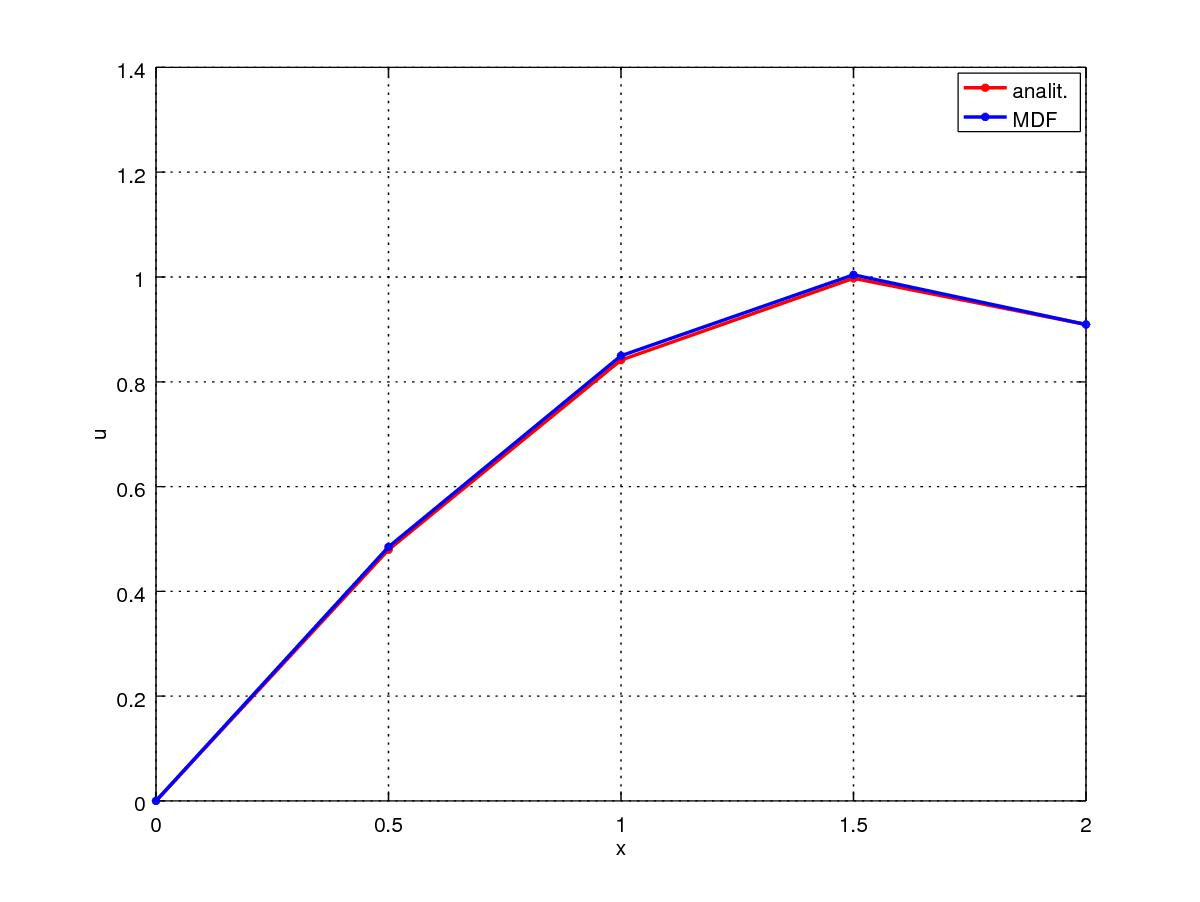
\includegraphics[width=0.8\textwidth]{./cap_pvc/dados/ex_pvc_mdf_1/ex_pvc_mdf_1}
  \caption{Resultado referente ao Exemplo~\ref{ex:pvc_mdf_1}.}
  \label{fig:ex_pvc_mdf_1}
\end{figure}

A solução analítica deste problema é $u(x) = \sen(x)$. Agora, usando a abordagem pelo método de diferenças finitas abordado nesta seção, obtemos o seguinte problema discreto
\begin{align}
  u_1 &= 0,\\
  -\frac{1}{h^2}u_{i-1} + \frac{2}{h^2}u_i - \frac{1}{h^2}u_{i+1} &= \sen(x_i),~i=2, \dotsc, n-1,\\
  u_n &= \sen(2),
\end{align}
onde $h=\pi/(n-1)$ e $x_i = (i-1)h$.

\begin{table}[h!]
  \centering
  \begin{tabular}{ll|c}
    $h$ & $n$ & $\|\tilde{u} - u\|_{L^2}$ \\\hline
    $10^{-1}$ & $21$ & $1,0\E-03$ \\
    $10^{-2}$ & $201$ & $3,3\E-05$ \\
    $10^{-3}$ & $2001$ & $1,0\E-06$ \\\hline
  \end{tabular}
  \caption{Resultados referentes ao Exemplo~\ref{ex:pvc_mdf_1}.}
  \label{tab:ex_pvc_mdf_1}
\end{table}

Resolvendo este sistema com $h=0,5$ obtemos a solução numérica apresentada na Figura~\ref{fig:ex_pvc_mdf_1}. Ainda, na Tabela~\ref{tab:ex_pvc_mdf_1} temos a comparação na norma $L^2$ da solução numérica $\tilde{u} = (u_1, u_2, \dotsc, u_n)$ com a solução analítica $u(x)=\sen(x)$ para diferentes escolhas de $h$.

\ifisoctave
No \verb+GNU Octave+, podemos computar os resultados discutidos neste exemplo com o seguinte código:
\begin{verbatim}
#param
n = 5;
h = 2/(n-1);

#fonte
f = @(x) sin(x);

#nodos
x = linspace(0,2,n)';

#sist. MDF
A = zeros(n,n);
b = zeros(n,1);

A(1,1) = 1;
b(1)=0;
for i=2:n-1
  A(i,i-1)=-1/h^2;
  A(i,i)=2/h^2;
  A(i,i+1)=-1/h^2;
  b(i)=sin(x(i));
endfor
A(n,n)=1;
b(n)=sin(2);

#sol MDF
u = A\b;

#sol. analic.
ua = @(x) sin(x);

#grafico comparativo
plot(x,ua(x),'r.-',...
     x,u,'b.-');grid
legend("analit.","MDF")
xlabel("x")
ylabel("u")

#erro na norma L2
printf("%1.1E %1.1E\n", h,norm(u-ua(x)))
\end{verbatim}
\fi
\end{ex}

\subsection*{Exercícios}

\begin{exer}
Considere o seguinte problema de valor inicial
  \begin{align}
    -u'' &+ u' = f(x),~-1<x<1,\\
    u(-1)&=0,\\
    u'(1)&=0,
  \end{align}
  onde
  \begin{equation}
    f(x) = \left\{
      \begin{array}{ll}
        1 &, x\leq 0\\
        0 &, x>0
      \end{array}
    \right.
  \end{equation}
\end{exer}
Use uma aproximação adequada pelo método de diferenças finitas para obter o valor aproximado de $u(0)$ com precisão de $2$ dígitos significativos.
\begin{resp}
  \ifisoctave 
  \href{https://github.com/phkonzen/notas/blob/master/src/MatematicaNumerica/cap_pvc/dados/exer_pvc_mdf_1/exer_pvc_mdf_1.m}{Código.} 
  \fi
  $7,2\E-1$
\end{resp}
